\documentclass[12pt]{article}

% Font family
\usepackage{xeCJK}
\setCJKmainfont{Noto Serif TC}
\usepackage{amssymb}
\usepackage{amsmath}

% Document layout
\usepackage[margin=2cm, a4paper]{geometry}
\usepackage{setspace}
\onehalfspacing
\setlength{\parskip}{12pt}
\setlength{\parindent}{0pt}

% Citation
\usepackage{biblatex}
\addbibresource{./ref.bib}

% Image
\usepackage{graphicx}
\graphicspath{{./images/}}

\author{\normalsize 施宇庭 NN6124030}
\date{}


\title{\Large AOC 2024 Spring - Lab 3 Hybrid Multiplier}

\begin{document}
\maketitle

\section{Implmenetation of Hybrid Multiplier}
% Pass TB0/TB1/TB2.Screenshot all pass screens.

\subsection*{Testbench 0 Passed}
\begin{figure}[h]
    \centering
    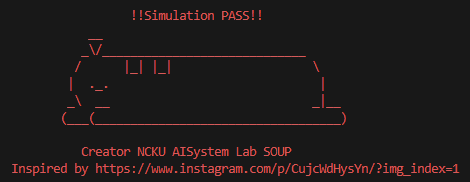
\includegraphics[width=0.4\linewidth]{./images/tb0.png}
\end{figure}

\subsection*{Testbench 1 Passed}
\begin{figure}[h]
    \centering
    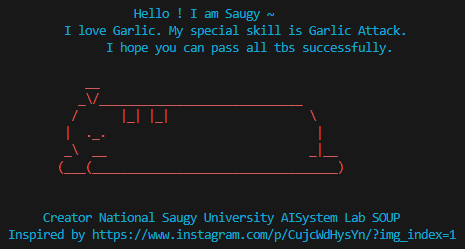
\includegraphics[width=0.4\linewidth]{./images/tb1.png}
\end{figure}

\subsection*{Testbench 2 Passed}
\begin{figure}[h]
    \centering
    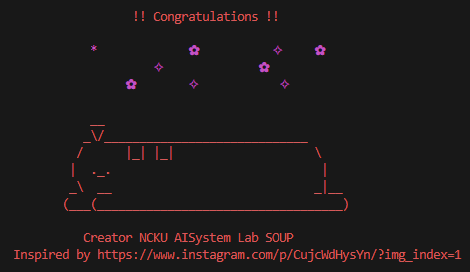
\includegraphics[width=0.4\linewidth]{./images/tb2.png}
\end{figure}

\section{Architecture and Algorithm}
% Explain how your multiplier works, its architecture and the algorithm you apply

這次的 hybrid multiplication 我選擇實作 Modified Booth's Algorithm,整個乘法器 (如 Figure \ref{fig:mul_arch1} 所示) 可以做 8-bit 和 8-bit 的有號整數乘法,輸出為一個 24-bit 的有號整數,由四個 Modified Booth Unit (MBU) 和一個 adder tree 組成。每個 MBU (如 Figure \ref{fig:mbu_arch} 所示) 由 3-bit 的 multiplier 來選擇輸出是 -2、-1、0、1 或 2 倍的 multiplicand,為了避免 overflow 輸出為 10 bits,並做 signed extension。

\begin{figure}[h]
    \centering
    \subfigure[Modified Booth Unit (MBU)]{
        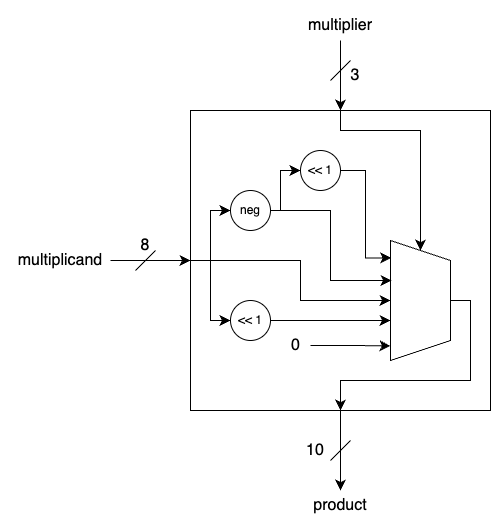
\includegraphics[width=0.4\textwidth]{mbu_arch.png}
        \label{fig:mbu_arch}
    }
    \hfill
    \subfigure[Hybrid multiplier using MBUs]{
        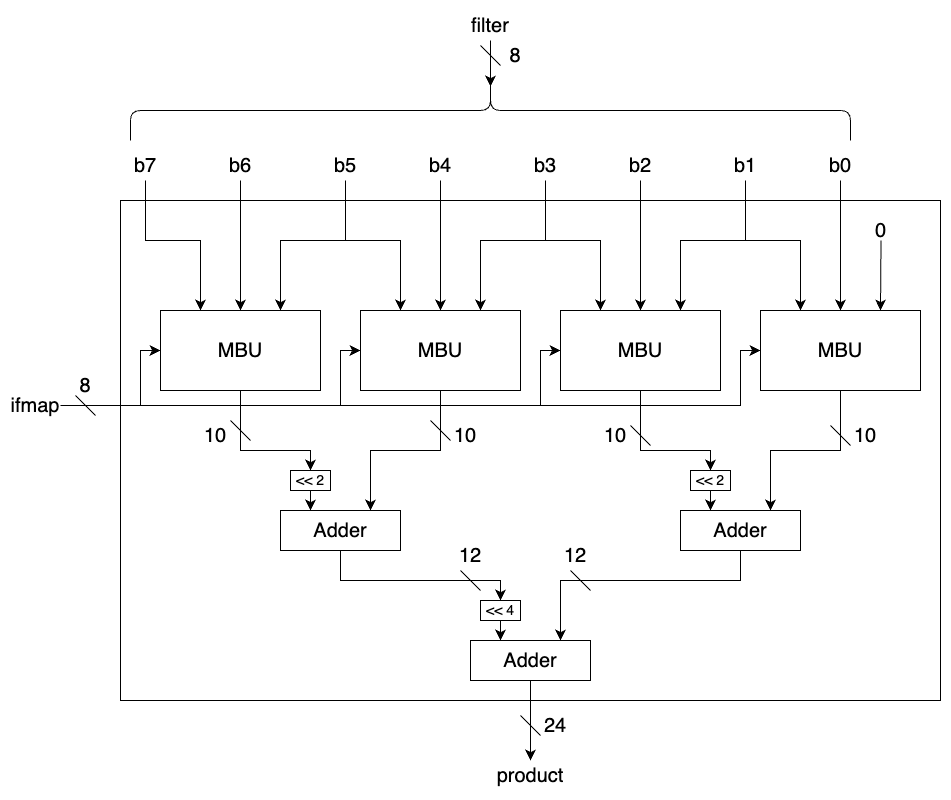
\includegraphics[width=0.5\textwidth]{mul_arch1.png}
        \label{fig:mul_arch1}
    }
    \caption{Hardware architecture of hybrid multiplier using Modified Booth's Algorithm.}
\end{figure}

\section{Hardware Reuse}
% Introduce each module and write down how do you reuse hardware resources to accomplish 3 testbenches

Figure \ref{fig:mul_arch1} 的輸出可作為 testbench 0 的答案,為了可以同時支援不同 bits 數的有號整數乘法,並盡可能重用既有的硬體,Figure \ref{fig:mul_arch2} 為修改後的 datapath,添加了 ifmap 和 filter 的 preprocessing units (圖中的 Prep 和 2-to-1 MUX),針對不同的 testbench 做 input 的前處理,四個 MBUs 的輸出個自取 [5:0] bits 拼接起來 (圖中左邊的 Concat) 即可作為 testbench 2 的答案,第一層 adder 的輸出拼接起來可作為 testbench 1 的答案,第二層 adder 的輸出做 signed extension 後則為 testbench 0 的答案。如此便成功重用了原本 Figure \ref{fig:mul_arch1} 架構中的 MBUs 和 adders。

\begin{figure}[h]
    \centering
    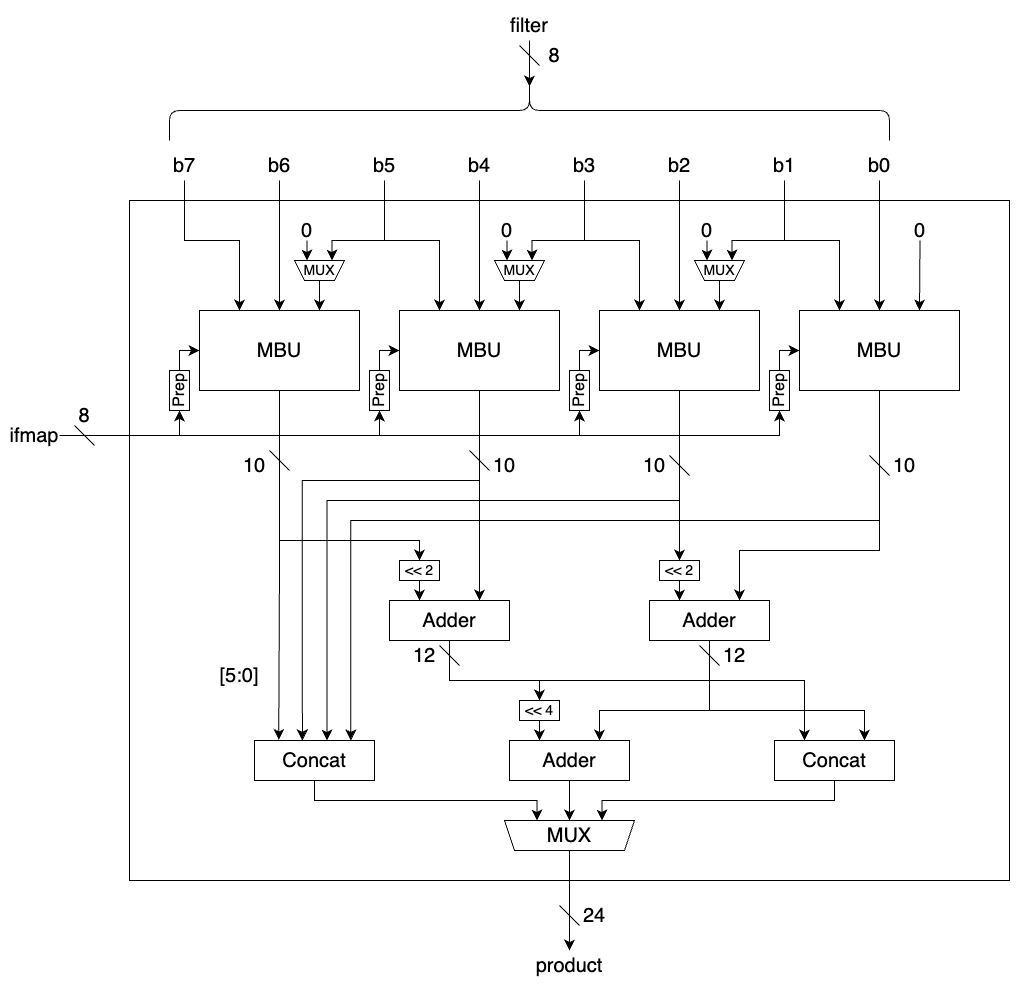
\includegraphics[width=0.7\textwidth]{mul_arch2.png}
    \caption{Hardware architecture of Modified Booth multiplier supporting 2-bit, 4-bit, and 8-bit signed integer multiplication.}
    \label{fig:mul_arch2}
\end{figure}
\newpage

\section{FLOPs and MACs in the 1st Layer of VGG19-Cifar10}
% How many (minimum) FLOPs and MACs does VGG16-Cifar10 1st layer require? Write down you calculation process. (without batch normalization and bias)

VGG-16 的第一層計算是 convolution,有 64 個 size 為 3x3 的 kernel,padding 為 1、padding 為 1,所以 input、output 和 kernel 的尺寸如 Table \ref{tab:conv} 所列。

\begin{table}[h]
    \centering
    \caption{The size of input, output, and kernel of the first convolution layer of VGG16-CIFAR10.}
    \begin{tabular}{cllll} \hline
           & Batch size & Channel & Height  & Width   \\ \hline
    Input  & $N=1$      & $C=3$   & $X=32$  & $X=32$  \\
    Kernel & $M=64$     & $C=3$   & $K=3$   & $K=3$   \\
    Output & $N=1$      & $M=64$  & $Y=32$  & $Y=32$  \\ \hline
    \end{tabular}
    \label{tab:conv}
\end{table}

% $$
% Y = 1 + \frac{X - K + 2 \times \text{padding}}{\text{stride}}
% $$

計算每個 output element 需要 $C \times K^2$ 個乘法,整個 output tensor 有 $N \times M \times Y^2$ 個 elements,因此總 MACs 數為:

$$
\text{MACs} \
= (N \times M \times Y^2) \times (C \times K^2) \
= (1 \times 64 \times 32^2) \times (3 \times 3^2) \
= 1769472
$$

計算每個 output element 需要 $C \times K^2$ 個乘法和 $C \times K^2 - 1$ 個加法,整個 output tensor 有 $N \times M \times Y^2$ 個 elements,因此總 FLOPs 數為:

$$
\text{FLOPs} \
= (N \times M \times Y^2) \times (C \times K^2 + C \times K^2 - 1) \
= (1 \times 64 \times 32^2) \times (3 \times 3^2 + 3 \times 3^2 - 1) \
= 3473408
$$

\section{FLOPs and MACs in a 512x10 Fully Connected Layer}
% How many (minimum) FLOPs and MACs does a fully connected (512-10) layer require? Write down your calculation process. (without batch normalization and bias)

\begin{table}[h]
    \centering
    \caption{The size of input, output, and kernel of a 512x10 fully connected layer.}
    \begin{tabular}{cll} \hline
           & Rows    & Columns  \\ \hline
    Input  & $M=512$  & $1$      \\
    Kernel & $N=10$ & $M=512$   \\
    Output & $N=10$ & $1$      \\ \hline
    \end{tabular}
    \label{tab:matmul}
\end{table}


計算每個 output element 需要 $M$ 個乘法,整個 output tensor 有 $N$ 個 elements,因此總 MACs 數為:

$$
\text{MACs} \
= N \times M \
= 10 \times 512 \
= 5120
$$

計算每個 output element 需要 $M$ 個乘法和 $M - 1$ 個加法,整個 output tensor 有 $N$ 個 elements,因此總 FLOPs 數為:

$$
\text{FLOPs} \
= N \times (M + M - 1) \
= 10 \times (512 + 512 - 1) \
= 10230
$$

\section{Difference between Hybrid Multiplier Algorithms}
% Compare the difference among using Robertson Algorithm, Booth Algorithm and Modified Booth Algorithm with Hybrid Multiplier with a table

三個乘法演算法大致上都可以分為兩個階段:

\begin{enumerate}
    \item 從 multiplier 取出數個 bits (以下稱為 select bits),用來決定輸入給下個階段的 partial sum 為幾倍的 multiplicand,若為有號數乘法,則產生 partial sum 的階段要做 signed extension
    \item 將所有的 partial sum 加起來,輸出最後結果為 product
\end{enumerate}

Robertson's Algorithm、Booth's Algorithm 和 Modified Booth's Algorithm 分別採用 1、2 和 3 個 select bits,select bits 數量越多代表第一階段會花費更多的硬體資源和計算時間,但會減少 partial sum 的數量,因此在第二階段可以節省硬體資源和計算時間。

三種演算法的差異主要體現在第一階段,與第二階段的作法的搭配是獨立的,可以使用傳統的 carry-propagate adders 或是 Wallace tree adder 等不同的作法,藉由平衡兩個階段的成本,在不同的場景下會有各自適合的演算法。以下 Table \ref{tab:algo_cmp} 為三種演算法的比較:

\begin{table}[h]
    \centering
    \caption{Comparison among Robertson's, Booth's and Modified Booth's algorithms}
    \begin{tabular}{|p{0.15\textwidth}|p{0.25\textwidth}|p{0.25\textwidth}|p{0.25\textwidth}|} \hline
     & Robertson & Booth & Modified Booth \\ \hline
    select bits & 1 bit & 2 bits & 3 bits \\ \hline
    partial sum & 和 multiplier bits 數量一樣 & 和 multiplier bits 數量一樣 & multiplier bits 數量的一半 \\ \hline
    計算時間 & 較長 &  multiplier 由連續 1/0 組成時有加速效果  & 減少 partial sum 數量,速度最快 \\ \hline
    硬體實作 & 簡單 & 需要 LUT,中等 & 需要更多 LUT,較複雜 \\ \hline
    適用場景 & 硬體資源受限的環境 & 需要快速計算的應用 & 高性能計算和大規模數據處理 \\ \hline
    \end{tabular}
    \label{tab:algo_cmp}
\end{table}

% \begin{table}[h]
%     \centering
%     \caption{Comparison among Robertson's, Booth's and Modified Booth's algorithms}
%     \begin{tabular}{|p{0.1\textwidth}|p{0.25\textwidth}|p{0.25\textwidth}|p{0.25\textwidth}|} \hline
%      & Robertson & Booth & Modified Booth \\ \hline
%     基本概念 & 簡單直觀的乘法演算法 & 二進位整數乘法的有效算法,特別是對於有符號的2的補數表示法 & 改進 Booth algorithm,通過編碼更多位來推斷乘數與被乘數的加法或減法的需要 \\ \hline
%     操作 & 進行加法或減法的迭代 & 乘數和被乘數的 partial sum 生成和累加 & 減少了生成 partial sum 的數量,通過將乘數分為2位一組來進行編碼 \\ \hline
%     效率 & 使用較少的硬體資源,但計算時間較長 & 計算時間較短,但可能需要更多的硬體資源 & 通過減少 partial sum 的數量來提高速度和性能 \\ \hline
%     適用性 & 適用於硬體資源受限的環境 & 適用於需要快速計算的應用 & 適用於高性能計算和大規模數據處理 \\ \hline
%     特點 & 硬體簡單,但速度較慢 & 處理速度快,但硬體複雜度較高 & 編碼技術減少了計算步驟,提高了計算速度 \\ \hline
%     \end{tabular}
%     % \label{tab:algo_cmp}
% \end{table}

\section{4-bit Signed Integer Multiplier using Wallace Tree}
% (Architecture 2) Design 4-bit & 4-bit multiplier (signed-number multiplication) with full and half
% adders follow architecture and point figure format in page 14. Introduce your architecture and
% method. Count and mark the latency/critical path of 4-bit & 4-bit multiplie
% (you can use Adder as time unit).

\subsection*{Algorithm}

講義中提供的 wallace tree multiplier 做的是 4-bit 無號整數的乘法,輸入為兩個 4-bit integer,輸出則為一個 8-bit integer,而 4-bit 的有號整數乘法,需要先將兩個 4-bit 的輸入擴展成 8-bit,再使用 Wallace Tree 進行乘法運算,如 Figure \ref{fig:wallace_algo1} 所示,其中每個小圓點是一個 bit,黃色是乘法器的輸入,粉色是 signed extension bits,藍色是加法器的 sum,綠色是加法器的 carry,帶有兩個原點的圓角方格代表半加器,三個原點的圓角方格則為全加器。

\begin{figure}[h]
    \centering
    \subfigure[Wallace Tree]{
        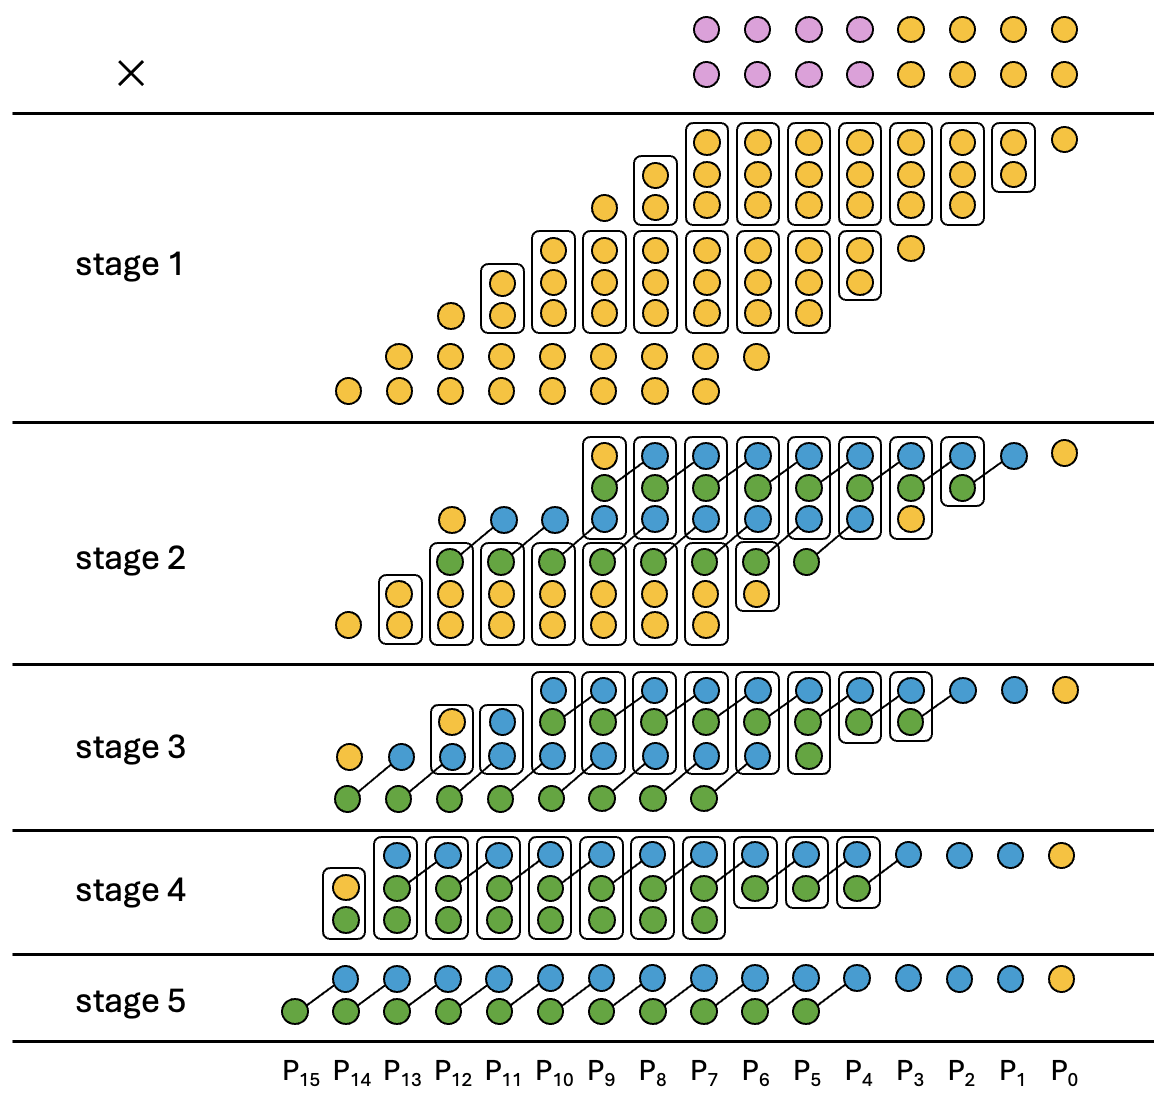
\includegraphics[width=0.38\textwidth]{wallace_algo1.png}
        \label{fig:wallace_algo1}
    }
    \hfill
    \subfigure[Optimized Wallace Tree]{
        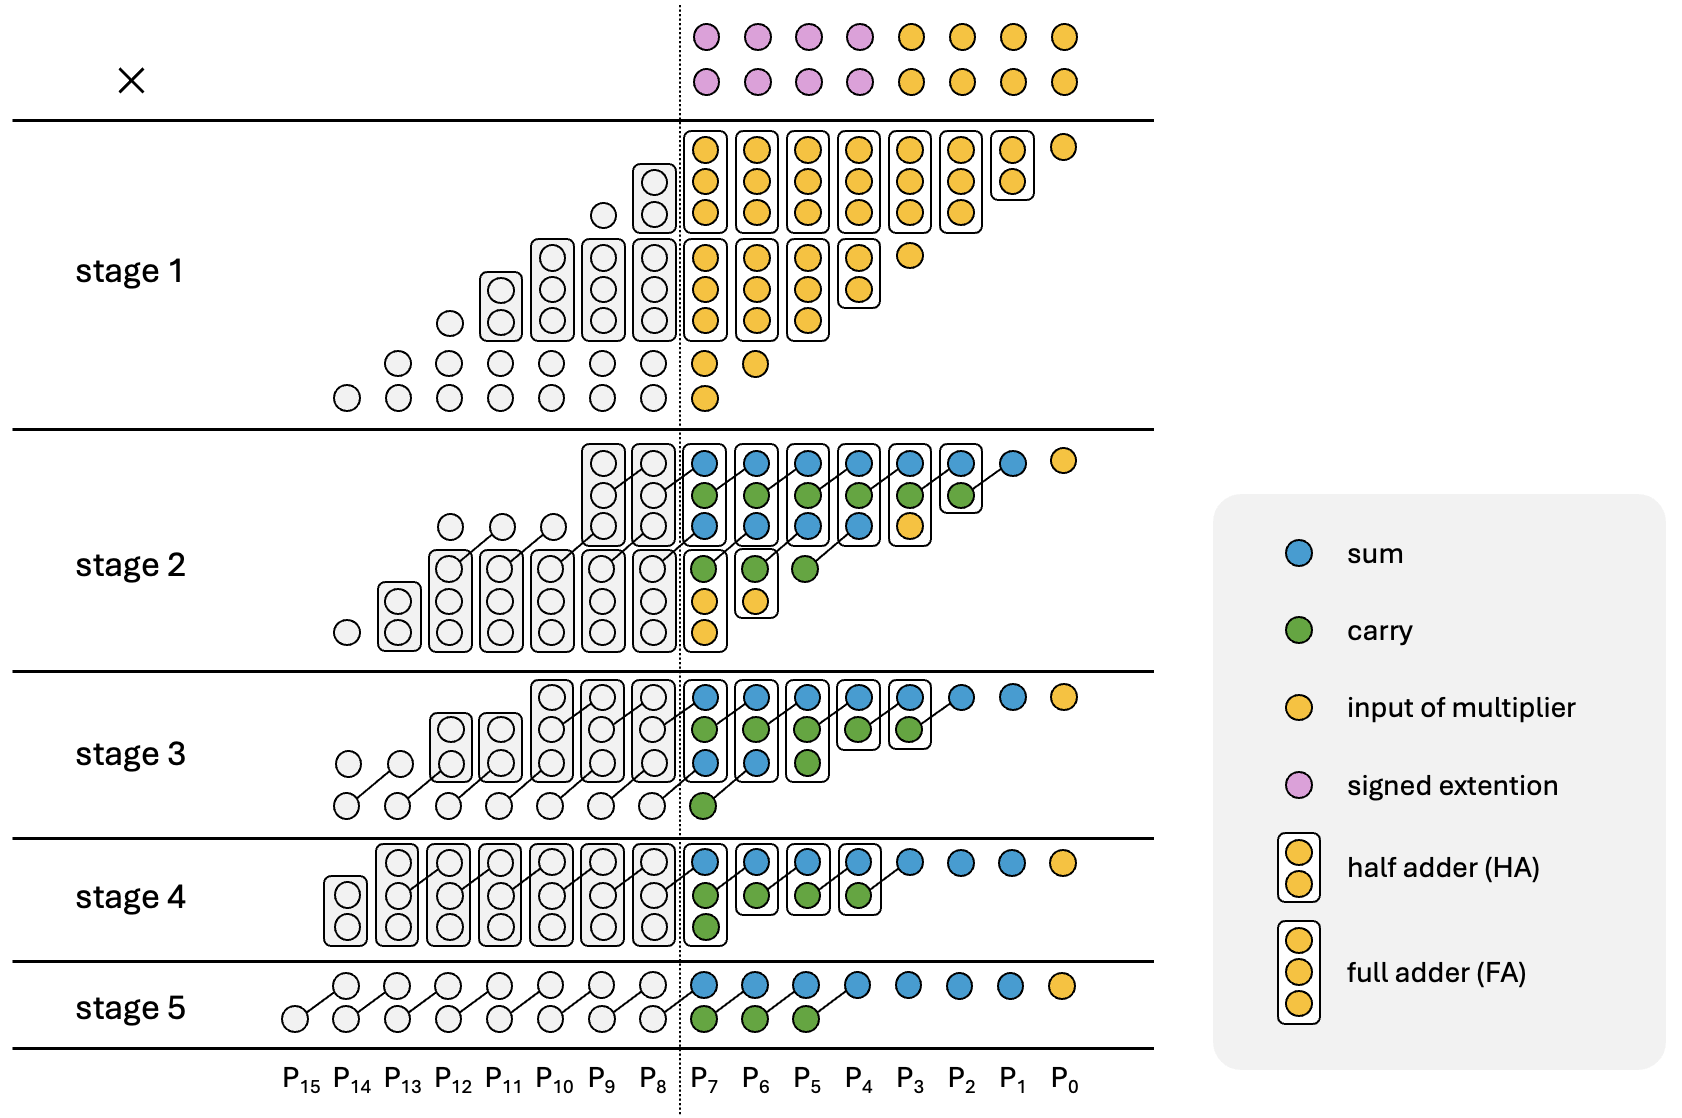
\includegraphics[width=0.55\textwidth]{wallace_algo2.png}
        \label{fig:wallace_algo2}
    }
    \caption{Algorithm of 4-bit signed integer multiplication using Wallace Tree.}
\end{figure}

Figure \ref{fig:wallace_algo1} 的演算法可以完成 4-bit 對 4-bit 的有號整數乘法,但仔細觀察可以發現,輸出的 16 bits 中其實只需要低位的 8 bits,因此如 Figure \ref{fig:wallace_algo2} 所呈現,左半邊的運算都不是必要的可以省略。

\subsection*{Architecture}

根據 Figure \ref{fig:wallace_algo2} 可以設計出 Figure \ref{fig:wallace_arch1} 的硬體,critical path 則發生在計算 bit $\text{P}_\text{7}$ 的路徑上,如 Figure \ref{fig:wallace_arch2} 所示,以紅色的線和紅色邊框的方塊來表示,其中一個全加器的 latency 等於兩個半加器的 latency 加上一個 OR gate 的 latency (如 Figure \ref{fig:adder} 所示),vector merging 的部分需要由三個全加器構成的 carry-propagate adder (CPA),因此在 critical path 上需要完整經過 6 層全加器和 1 層半加器的 latency。

\begin{figure}[h]
    \centering
    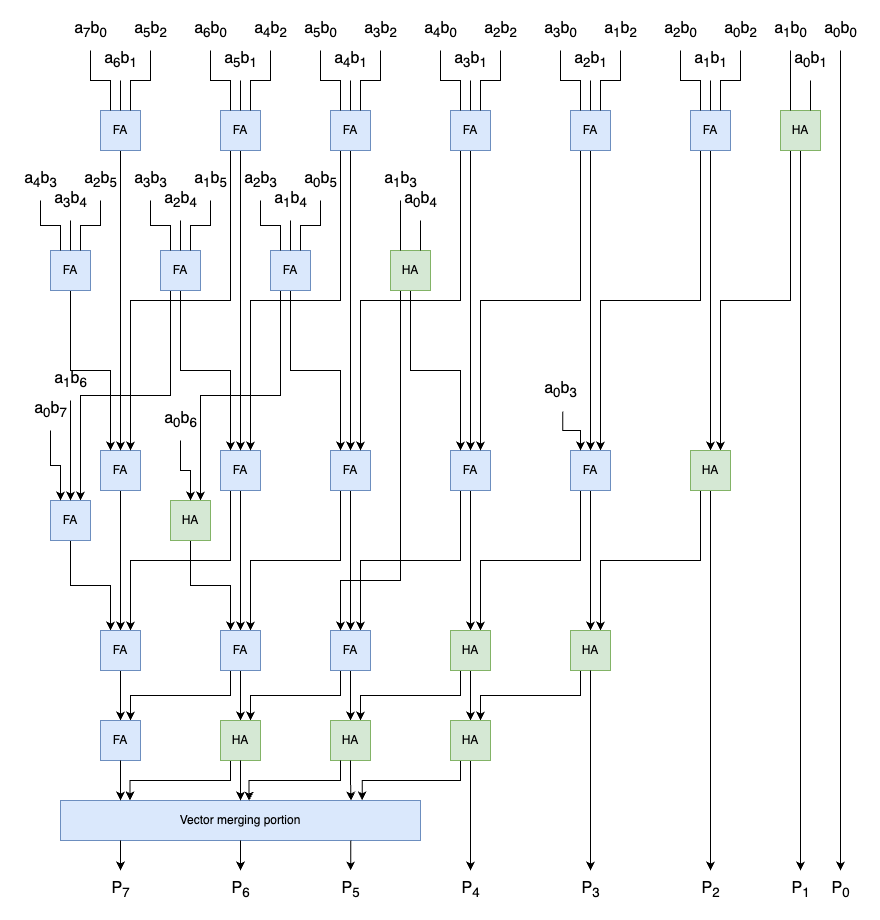
\includegraphics[width=0.6\textwidth]{wallace_arch1.png}
    \caption{Hardware architecture of 4-bit signed integer multiplier using Optimized Wallace Tree.}
    \label{fig:wallace_arch1}
\end{figure}

\begin{figure}[h]
    \centering
    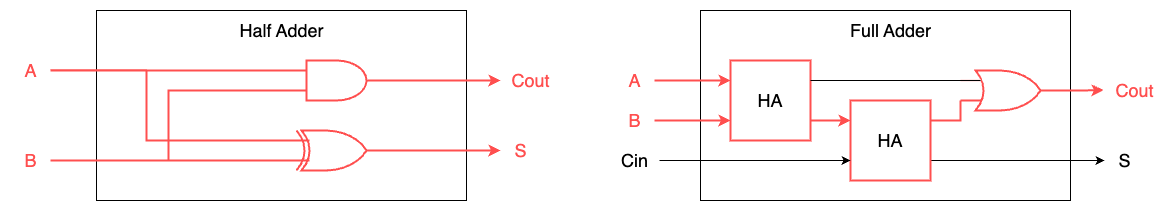
\includegraphics[width=0.8\textwidth]{adder.png}
    \caption{Critical paths of half adder and full adder (shown as red wires and blocks). The latency of a full adder is 3x of the latency of a half adder.}
    \label{fig:adder}
\end{figure}

\begin{figure}[h]
    \centering
    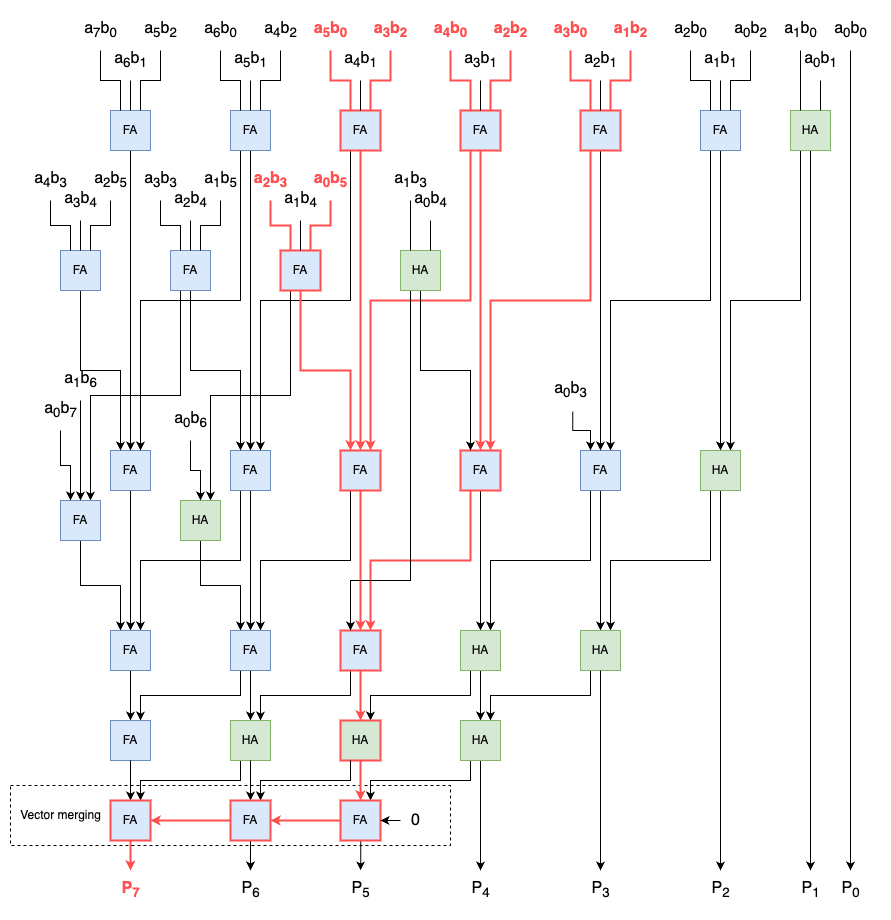
\includegraphics[width=0.6\textwidth]{wallace_arch2.png}
    \caption{Critical path of 4-bit signed integer multiplier using Optimized Wallace Tree (shown as red wires and blocks).}
    \label{fig:wallace_arch2}
\end{figure}

\newpage

\section{Thoughts and Advices}
% Share your thoughts on this lab. Any takeaways or advices? Or anything you want to say

\begin{enumerate}
    \item 這次的 lab 自己設計乘法器滿有趣的,以往計組最多只學到 Robertson algorithm 和 Booth algorithm,但這次的 lab 還介紹了其他的作法和優化技巧,包括 Modified Booth's algorithm 和 Wallace Tree,收穫很多。
    \item 這次 lab 但在環境上花了不少時間,助教推薦用的 MobaXTerm 只支援 Windows 系統,但 macOS 和 Linux 都無法安裝,如果可以的話希望未來助教在準備與測試開發環境時能多考量到使用不同作業系統的同學。
    \item Makefile 有 redundant 的部分,可以寫得更精簡,不只乘法器 hardware 要 reuse,Makefile 指令也應該要 reuse。
\end{enumerate}

\end{document}
